\section{DT Block Diagrams}

\subsection{The Four Basic Motifs}

Block diagrams of DT systems are similar to CT systems.

The four motifs are:

\begin{itemize}
\item A single block.\\[1em] 
\begin{tikzpicture}[auto, node distance=2cm,>=latex',scale=1, every node/.style={transform shape}]
    \node [input, name=input] {};
    \node [block, right of=input] (system) {$\mathcal{S}_1$};
    \node [output, right of=system] (output) {};


    \draw [draw,->] (input) -- node {$x[n]$} (system);
    \draw [->] (system) -- node {$y[n]$} (output);
\end{tikzpicture}

\item A {\it series} connection of two blocks\\[1em]
\begin{tikzpicture}[auto, node distance=2cm,>=latex',scale=1, every node/.style={transform shape}]

    \node [input, name=input] {};
    \node [block, right of=input] (system1) {$\mathcal{S}_1$};
    \node [block, right of=system1,node distance=4cm] (system2) {$\mathcal{S}_2$};
    \node [output, right of=system2] (output) {};


    \draw [draw,->] (input) -- node {$x[n]$} (system1);
    \draw [->] (system1) -- (system2);
    \draw [->] (system2) -- node {$y[n]$} (output);
\end{tikzpicture}
\item A {\it parallel} connection of two blocks\\[1em]
\begin{tikzpicture}[auto, node distance=2cm,>=latex',scale=1, every node/.style={transform shape}]

    \node[shape=coordinate] at (1,1) (input1) {};
    \node[block] at (3,1) (block1) {$\mathcal{S}_1$};
    \node[shape=coordinate] at ($(block1.east)+(0.5,0)$) (output1) {};
    \draw[->] (input1) -- (block1);
    \draw (block1) -- (output1);

    \node[shape=coordinate] at (1,-1) (input2) {};
    \node[block] at (3,-1) (block2) {$\mathcal{S}_2$};
    \node[shape=coordinate] at ($(block2.east)+(0.5,0)$) (output2) {};
    \draw[->] (input2) -- (block2);
    \draw (block2) -- (output2);

    \node [input, name=input] at (0,0) {};  	
    \node [input, name=conn] at (1,0) {};
    \draw (conn) -- (input1);
    \draw (conn) -- (input2);
    \node [sum, right of=input,node distance=5cm] (sum) {$\Sigma$};
    \draw [->] (output1) -| (sum);
    \draw [->] (output2) -| (sum);

    \draw [draw] (input) -- node {$x[n]$} (conn);
    \node [output, right of=sum] (output) {};
    \draw [->] (sum) -- node {$y[n]$} (output);
\end{tikzpicture}

\item A {\it feedback} connection\\[1em]
\begin{tikzpicture}[auto, node distance=2cm,>=latex',scale=1, every node/.style={transform shape}]
    \node[block] at (4,0) (block1) {$\mathcal{S}_1$};

    \node[block] at (4,-2) (block2) {$\mathcal{S}_2$};
    \node[shape=coordinate] at (6,-2) (input2) {};

    \node [input, name=input] at (0,0) {};  	
    \node [shape=coordinate, name=conn] at (6,0) {};
    \draw (block1) -- (conn);
    \draw (conn) -- (input2);
    \draw [->] (input2) -- (block2);

    \node [sum, right of=input,node distance=2cm] (sum) {$\Sigma$};
    \draw [->] (block2) -| node[pos=0.95] {$-$} (sum);

    \draw [draw,->] (input) -- node {$x[n]$} (sum);
    \draw [->] (sum) -- (block1);
    \node [output, right of=conn] (output) {};
    \draw [->] (conn) -- node {$y[n]$} (output);
\end{tikzpicture}
\end{itemize}

Note the feedback is negative (the minus sign on the feedback summation input). As in CT, these can be use in various combinations.

\subsection{Connections to Convolution}

Each subsystem, $\mathcal{S}_i$, can be represented by a basic discrete time-domain operation (e.g. differences, running sums, addition, and scaling) or more generally by it's impulse response $h_i[n]$.

For example a block representing an system acting as a delay of one sample is typically drawn as

\begin{center}
  \begin{tikzpicture}[auto, node distance=2cm,>=latex',scale=1, every node/.style={transform shape}]
    \node [input, name=input] {};
    \node [block, right of=input] (system) {$D$};
    \node [output, right of=system] (output) {};
    \draw [draw,->] (input) -- node {$x[n]$} (system);
    \draw [->] (system) -- node[pos=2] {$y[n] = x[n-1]$} (output);
\end{tikzpicture}
\end{center}
This is equivalent to an impulse response $h[n] = \delta[n-1]$ so that it might also be drawn as
\begin{center}
  \begin{tikzpicture}[auto, node distance=2cm,>=latex',scale=1, every node/.style={transform shape}]
    \node [input, name=input] {};
    \node [block, right of=input] (system) {$h[n] = \delta[n-1]$};
    \node [output, right of=system] (output) {};

    \draw [draw,->] (input) -- node {$x[n]$} (system);
    \draw [->] (system) -- node[pos=4] {$y[n] = x[n] * \delta[n-1] = x[n-1]$} (output);
\end{tikzpicture}
\end{center}

Similarly, a block representing an system acting as an advance of one sample is typically drawn as

\begin{center}
  \begin{tikzpicture}[auto, node distance=2cm,>=latex',scale=1, every node/.style={transform shape}]
    \node [input, name=input] {};
    \node [block, right of=input] (system) {$E$};
    \node [output, right of=system] (output) {};
    \draw [draw,->] (input) -- node {$x[n]$} (system);
    \draw [->] (system) -- node[pos=2] {$y[n] = x[n+1]$} (output);
\end{tikzpicture}
\end{center}
This is equivalent to an impulse response $h[n] = \delta[n+1]$ so that it might also be drawn as
\begin{center}
  \begin{tikzpicture}[auto, node distance=2cm,>=latex',scale=1, every node/.style={transform shape}]
    \node [input, name=input] {};
    \node [block, right of=input] (system) {$h[n] = \delta[n+1]$};
    \node [output, right of=system] (output) {};

    \draw [draw,->] (input) -- node {$x[n]$} (system);
    \draw [->] (system) -- node[pos=4] {$y[n] = x[n] * \delta[n+1] = x[n+1]$} (output);
\end{tikzpicture}
\end{center}

We can use the concept of convolution to connect block diagrams to the properties of convolution

\begin{itemize}
\item A single block is equivalent to convolution with the impulse response for that subsystem\\[1em] 
\begin{tikzpicture}[auto, node distance=2cm,>=latex',scale=1, every node/.style={transform shape}]

    \node [input, name=input] {};
    \node [block, right of=input] (system) {$h_1[n]$};
    \node [output, right of=system] (output) {};

    \draw [draw,->] (input) -- node {$x[n]$} (system);
    \draw [->] (system) -- node[pos=2] {$y[n] = h_1[n]*x[n]$} (output);
\end{tikzpicture}

\item Using the associative property, a series connection of two blocks becomes
  \begin{center}
\begin{tikzpicture}[auto, node distance=2cm,>=latex',scale=1, every node/.style={transform shape}]
    % We start by placing the blocks
    \node [input, name=input] {};
    \node [block, right of=input] (system1) {$h_1[n]$};
    \node [block, right of=system1,node distance=4cm] (system2) {$h_2[n]$};
    \node [output, right of=system2] (output) {};

    \draw [draw,->] (input) -- node {$x[n]$} (system1);
    \draw [->] (system1) -- (system2);
    \draw [->] (system2) -- node[pos=3] {$y[n] = \left(h_1[n]*h_2[n]\right)*x[n]$} (output);
\end{tikzpicture}
  \end{center}
  which can be reduced to a single convolution $y[n] = h_3[n]*x[n]$ where $h_3[n] = h_1[n]*h_2[n]$.
\item Using the distributive property, a parallel connection of two blocks becomes
  \begin{center}
\begin{tikzpicture}[auto, node distance=2cm,>=latex',scale=1, every node/.style={transform shape}]

    \node[shape=coordinate] at (1,1) (input1) {};
    \node[block] at (3,1) (block1) {$h_1[n]$};
    \node[shape=coordinate] at ($(block1.east)+(0.5,0)$) (output1) {};
    \draw[->] (input1) -- (block1);
    \draw (block1) -- (output1);

    \node[shape=coordinate] at (1,-1) (input2) {};
    \node[block] at (3,-1) (block2) {$h_2[n]$};
    \node[shape=coordinate] at ($(block2.east)+(0.5,0)$) (output2) {};
    \draw[->] (input2) -- (block2);
    \draw (block2) -- (output2);

    \node [input, name=input] at (0,0) {};  	
    \node [input, name=conn] at (1,0) {};
    \draw (conn) -- (input1);
    \draw (conn) -- (input2);
    \node [sum, right of=input,node distance=5cm] (sum) {$\Sigma$};
    \draw [->] (output1) -| (sum);
    \draw [->] (output2) -| (sum);

    \draw [draw] (input) -- node {$x[n]$} (conn);
    \node [output, right of=sum] (output) {};
    \draw [->] (sum) -- node[pos=3] {$y[n]= \left(h_1[n]*x[n]\right) +  \left(h_2[n]*x[n]\right) =  \left(h_1[n]+h_2[n]\right)*x[n]$} (output);
\end{tikzpicture}  
  \end{center}
  which is equivalent to a single convolution $y[n] = h_3[n]*x[n]$ where $h_3[n] = h_1[n] + h_2[n]$.
\item In the feedback connection let $w[n]$ be the output of the summation
  \begin{center}
\begin{tikzpicture}[auto, node distance=2cm,>=latex',scale=1, every node/.style={transform shape}]
    % We start by placing the blocks
    \node[block] at (4.5,0) (block1) {$h_1[n]$};

    \node[block] at (4,-2) (block2) {$h_2[n]$};
    \node[shape=coordinate] at (6,-2) (input2) {};

    \node [input, name=input] at (0,0) {};  	
    \node [shape=coordinate, name=conn] at (6,0) {};
    \draw (block1) -- (conn);
    \draw (conn) -- (input2);
    \draw [->] (input2) -- (block2);

    \node [sum, right of=input,node distance=2cm] (sum) {$\Sigma$};
    \draw [->] (block2) -| node[pos=0.95] {$-$} (sum);

    \draw [draw,->] (input) -- node {$x[n]$} (sum);
    \draw [->] (sum) -- (block1);
    \node [output, right of=conn] (output) {};
    \draw [->] (conn) -- node {$y[n]$} (output);
    \draw node at (3,0.3) {$w[n]$};
\end{tikzpicture}
  \end{center}
  Then $y[n] = h_1[n]*w[n]$ and $w[n] = x[n] - h_2[n]*y[n]$. Substituting the later into the former gives $y[n] = h_1*(x-h_2[n]*y[n])$. Using the distributive property we get $y[n] = h_1[n]*x[n] - h_1[n]*h_2[n]*y[n]$. Isolating the input on the right-hand side and using $y[n] = \delta[n]*y[n]$ we get
  \[
  y[n] + h_1[n]*h_2[n]*y[n] = \left(\delta[n] + h_1[n]*h_2[n]\right)*y[n] = h_1[n]*x[n] 
  \]
  We can solve this for $y[n]$ using the concept of inverse systems. Let $h_3[n]* \left(\delta[n] + h_1[n]*h_2[n]\right)= \delta[n]$, i.e. $h_3$ is the inverse system of $\delta[n] + h_1[n]*h_2[n]$. Then
  \[
  y[n] = h_3[n]*h_1[n]*x[n]
  \]
\end{itemize}

Recall, when the system is instantaneous (memoryless) the impulse response is $a\delta[n]$ for some constant $a$. This is the same as scaling the signal by $a$. We typically drop the block in such cases and draw the input-output operation as

\begin{center}
\begin{tikzpicture}[auto, node distance=2cm,>=latex',scale=1, every node/.style={transform shape}]
  \node [input, name=input] at (0,0) {};
  \node [output, name=system] at (2,0) {};
  \node [output, name=output] at (4,0) {};
  \draw [draw,->] (input) -- node {$x[n]$} (system);
  \draw [draw,->] (system) -- node[pos=1] {$y[n] = ax[n]$} (output);
  \draw [->] (input) -- node {$a$} (output);
\end{tikzpicture}
\end{center}

These properties allow us to perform transformations, either breaking up a system into subsystems, or reducing a system to a single block.

\begin{example}
  Consider a second-order system system with impulse response
  \[
  h[n] = \left(\frac{1}{2}\right)^n\, u[n] + \left(\frac{3}{4}\right)^n\, u[n]
  \]
  We can express this as a block diagram consisting of two parallel blocks
  \begin{center}
\begin{tikzpicture}[auto, node distance=2cm,>=latex',scale=1, every node/.style={transform shape}]

    \node[shape=coordinate] at (1,1) (input1) {};
    \node[block] at (3,1) (block1) {$h_1[n] = \left(\frac{1}{2}\right)^nu[n]$};
    \node[shape=coordinate] at ($(block1.east)+(0.5,0)$) (output1) {};
    \draw[->] (input1) -- (block1);
    \draw (block1) -- (output1);

    \node[shape=coordinate] at (1,-1) (input2) {};
    \node[block] at (3,-1) (block2) {$h_2[n] = \left(\frac{3}{4}\right)^nu[n]$};
    \node[shape=coordinate] at ($(block2.east)+(0.5,0)$) (output2) {};
    \draw[->] (input2) -- (block2);
    \draw (block2) -- (output2);

    \node [input, name=input] at (0,0) {};  	
    \node [input, name=conn] at (1,0) {};
    \draw (conn) -- (input1);
    \draw (conn) -- (input2);
    \node [sum, right of=input,node distance=5cm] (sum) {$\Sigma$};
    \draw [->] (output1) -| (sum);
    \draw [->] (output2) -| (sum);

    \draw [draw] (input) -- node {$x[n]$} (conn);
    \node [output, right of=sum] (output) {};
    \draw [->] (sum) -- node[pos=1] {$y[n]$} (output);
\end{tikzpicture}
  \end{center}
\end{example}

\subsection{Connections to LCCDE}

The other DT system representation we have seen are linear, constant-coefficient difference equations. These can be expressed as combinations of advance or delay blocks. This is straightforward compared the CT system case.

\subsubsection*{First-Order System}

To illustrate this consider the first-order LCCDE
\[
y[n+1] + ay[n]= x[n+1]
\]
We can solve this for $y[n]$
\[
y[n] = -\frac{1}{a}y[n+1]  + \frac{1}{a}x[n+1]
\]
and can express this as a feedback motif using the advance operator $E$
\begin{center}
  \tikzstyle{block} = [draw, fill=gray!20, rectangle, 
      minimum height=2em, minimum width=2em]
  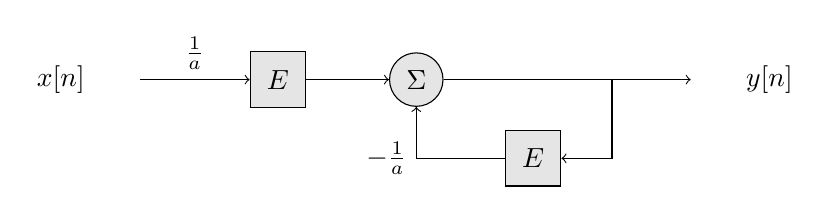
\begin{tikzpicture}[auto]
    \node [input, name=input] at (0,0) {};
    \node [left of=input] {$x[n]$};
    \node[block, right of=input, node distance=5em] (block1) {$E$};
    \node [sum, right of=block1, node distance=5em] (sum) {$\Sigma$};
    \node[block] at (5,-1) (block2) {$E$};
    \node [shape=coordinate, name=conn] at (6,0) {};
    \node[shape=coordinate] at (7,0) (output) {};
    \node [right of=output] {$y[n]$};
    
    \draw [->] (input) -- node {$\frac{1}{a}$} (block1);
    \draw [->] (block1) -- (sum);
    \draw (sum) -- (conn);
    \draw [->] (conn) -- (output);
    \draw [->] (conn) |- (block2);
    \draw [->] (block2) -| node {$-\frac{1}{a}$} (sum);
  \end{tikzpicture}
\end{center}

Alternatively we could rewrite the difference equation in recursive delay form
\[
y[n] = -ay[n-1] +x[n]
\]
which can be expressed as a block diagram using the delay operator, $D$
\begin{center}
  \tikzstyle{block} = [draw, fill=gray!20, rectangle, 
      minimum height=2em, minimum width=2em]
  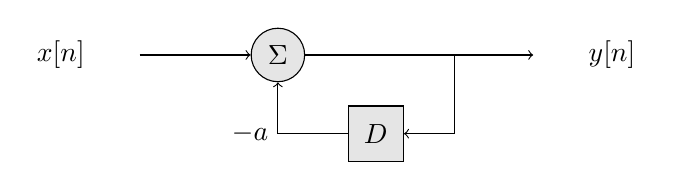
\begin{tikzpicture}[auto]
    \node [input, name=input] at (0,0) {};
    \node [left of=input] {$x[n]$};
    \node [sum, right of=input, node distance=5em] (sum) {$\Sigma$};
    \node[block] at (3,-1) (block2) {$D$};
    \node [shape=coordinate, name=conn] at (4,0) {};
    \node[shape=coordinate] at (5,0) (output) {};
    \node [right of=output] {$y[n]$};
    
    \draw [->] (input) -- (sum);
    \draw (sum) -- (conn);
    \draw [->] (conn) -- (output);
    \draw [->] (conn) |- (block2);
    \draw [->] (block2) -| node {$-a$} (sum);
  \end{tikzpicture}
\end{center}

The choice of using advance or delay blocks results in a non-causal or causal (respectively) system. Thus, delay blocks are required for real-time DT system implementations.

\subsubsection*{Second-Order System}

Now consider the second-order system
\[
y[n+2] + ay[n+1] + by[n] = x[n+2]
\]
Again, writing in recursive delay form 
\[
y[n] = -ay[n-1] - by[n-2] + x[n]
\]
we obtain the block diagram
\begin{center}
  \tikzstyle{block} = [draw, fill=gray!20, rectangle, 
      minimum height=2em, minimum width=2em]
  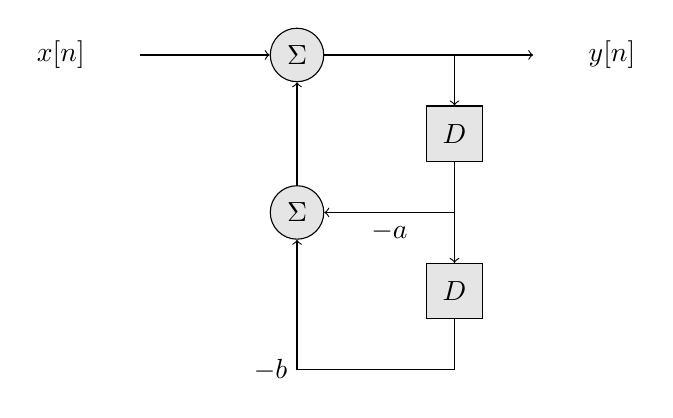
\begin{tikzpicture}[auto]
    \node [input, name=input] at (0,0) {};
    \node [left of=input] {$x[n]$};
    \node [sum] at (2,0) (sum1) {$\Sigma$};
    \node [block] at (4,-1) (block1) {$D$};
    \node [block] at (4,-3) (block2) {$D$};
    \node [shape=coordinate, name=conn1] at (4,-2) {};
    \node [shape=coordinate, name=conn2] at (4,-4) {};
    \node [sum] at (2,-2) (sum2) {$\Sigma$};
    \node [shape=coordinate, name=conn] at (4,0) {};
    \node [shape=coordinate] at (5,0) (output) {};
    \node [right of=output] {$y[n]$};
    
    \draw [->] (input) -- (sum1);
    \draw (sum1) -- (conn);
    \draw [->] (conn) -- (output);
    \draw [->] (conn) -- (block1);
    \draw (block1) -- (conn1);
    \draw [->] (conn1) -- node {$-a$} (sum2);
    \draw [->] (conn1) -- (block2);
    \draw (block2) -- (conn2);
    \draw [->] (conn2) -| node {$-b$} (sum2);
    \draw [->] (sum2) -- (sum1);
  \end{tikzpicture}
\end{center}

\subsection{Implementing a DT System}

As in the CT case, one of the most powerful uses of block diagrams is the implementation of a DT system in hardware. As we shall see later in the semester, designing a DT system for a particular purpose leads to a mathematical description that is equivalent to either an impulse response or a LCCDE. We have seen how these can be represented as block diagrams. Once we have reduced a system to blocks consisting of simple operations, we can then convert the block diagram to a digital circuit, implement using a digital signal processor, or write an equivalent program to run on an embedded or general purpose computer.

\begin{tabular}{cc}

  Block & Typical Digital Circuit\\
  \hline
  \tikzstyle{block} = [draw, fill=gray!20, rectangle, 
    minimum height=2em, minimum width=2em]
  \tikzstyle{sum} = [draw, fill=gray!20, circle, node distance=1cm]
  \tikzstyle{input} = [coordinate]
  \tikzstyle{output} = [coordinate]
  \tikzstyle{pinstyle} = [pin edge={to-,thin,black}]
  
  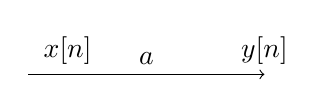
\begin{tikzpicture}[auto]
    \node [input, name=input] at (0,0) {};
    \node [shape=coordinate, name=signal1] at (1,0) {};
    \node [shape=coordinate, name=signal2] at (2,0) {};
    \node [output, right of=signal2] (output) {};

    \draw (input) -- node {$x[n]$} (signal1);
    \draw (signal1) -- node {$a$} (signal2);
    \draw [->] (signal2) -- node[pos=1] {$y[n]$} (output);
  \end{tikzpicture}  

  &
  Multiplier (ALU)
  \\[2em]

  \tikzstyle{block} = [draw, fill=gray!20, rectangle, 
    minimum height=2em, minimum width=2em]
  \tikzstyle{sum} = [draw, fill=gray!20, circle, node distance=1cm]
  \tikzstyle{input} = [coordinate]
  \tikzstyle{output} = [coordinate]
  \tikzstyle{pinstyle} = [pin edge={to-,thin,black}]
  
  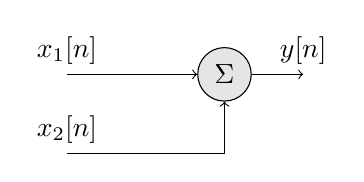
\begin{tikzpicture}[auto]
    \node [input, name=input1] at (0,0) {};
    \node [input, name=input2] at (0,-1) {};
    \node [sum] at (2,0) (sum1) {$\Sigma$};
    \node [output, right of=sum1] (output) {};
    
    \draw [->] (input1) -- node[pos=0] {$x_1[n]$} (sum1);
    \draw [->] (input2) -| node[pos=0] {$x_2[n]$} (sum1);
    \draw [->] (sum1) -- node[pos=1] {$y[n]$} (output);
  \end{tikzpicture}  
  &
  Adder (ALU)
  \\[2em]
      
  \tikzstyle{block} = [draw, fill=gray!20, rectangle, 
    minimum height=2em, minimum width=2em]
  \tikzstyle{sum} = [draw, fill=gray!20, circle, node distance=1cm]
  \tikzstyle{input} = [coordinate]
  \tikzstyle{output} = [coordinate]
  \tikzstyle{pinstyle} = [pin edge={to-,thin,black}]
  
  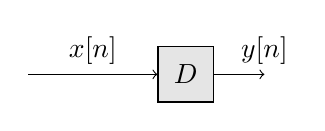
\begin{tikzpicture}[auto]
    \node [input, name=input] at (0,0) {};
    \node[block] at (2,0) (block1) {$D$};
    \node [output, right of=block1] (output) {};

    \draw [->] (input) -- node {$x[n]$} (block1);
    \draw [->] (block1) -- node[pos=1] {$y[n]$} (output);
  \end{tikzpicture}  

  &
  Shift Register\\
  \hline
\end{tabular}

\begin{example} The following C++ code implements the second order system given by
\begin{center}
  \tikzstyle{block} = [draw, fill=gray!20, rectangle, 
      minimum height=2em, minimum width=2em]
  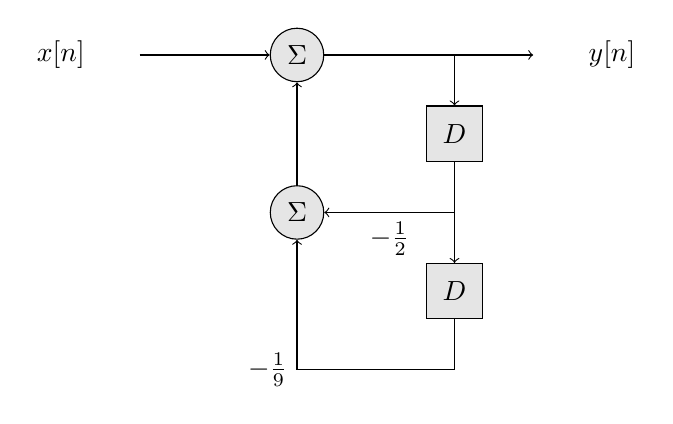
\begin{tikzpicture}[auto]
    \node [input, name=input] at (0,0) {};
    \node [left of=input] {$x[n]$};
    \node [sum] at (2,0) (sum1) {$\Sigma$};
    \node [block] at (4,-1) (block1) {$D$};
    \node [block] at (4,-3) (block2) {$D$};
    \node [shape=coordinate, name=conn1] at (4,-2) {};
    \node [shape=coordinate, name=conn2] at (4,-4) {};
    \node [sum] at (2,-2) (sum2) {$\Sigma$};
    \node [shape=coordinate, name=conn] at (4,0) {};
    \node [shape=coordinate] at (5,0) (output) {};
    \node [right of=output] {$y[n]$};
    
    \draw [->] (input) -- (sum1);
    \draw (sum1) -- (conn);
    \draw [->] (conn) -- (output);
    \draw [->] (conn) -- (block1);
    \draw (block1) -- (conn1);
    \draw [->] (conn1) -- node {$-\frac{1}{2}$} (sum2);
    \draw [->] (conn1) -- (block2);
    \draw (block2) -- (conn2);
    \draw [->] (conn2) -| node {$-\frac{1}{9}$} (sum2);
    \draw [->] (sum2) -- (sum1);
  \end{tikzpicture}
\end{center}
using floating point calculations. It assumes the current input is obtained via the function \texttt{read}, and the output written using the function \texttt{write}. The delayed values of the output are stored in the array \texttt{buffer} and are initialized to zero ("at rest" prior to application of the input).
\begin{verbatim}
double buffer[2] = {0.0,0.0};
while(true){
  double x = read();
  double y = -0.5*buffer[1] - buffer[0]/9.0 + x;
  write(y);
  buffer[0] = buffer[1];
  buffer[1] = y;
}
\end{verbatim}
Note in real applications it is common to replace the floating point calculations with fixed-width (scaled integer) ones.
$\blacksquare$
\end{example}

